\section{Reformulating the Standard Model Lagrangian in VAM Units}\label{sec:lagrangian_vam}

The Standard Model Lagrangian encapsulates particle dynamics through symmetry-based field terms:
\begin{equation}
    \mathcal{L}_{\text{SM}} = -\frac{1}{4}F^{\mu\nu}F_{\mu\nu} + i\bar{\psi}\gamma^\mu D_\mu \psi + y_f \bar{\psi}\phi \psi + |D_\mu \phi|^2 - V(\phi)
\end{equation}
While mathematically elegant, these terms are not derived from first physical principles but are inserted axiomatically. The Vortex \AE{}ther Model (VAM) replaces this abstraction with a Lagrangian based on vortex dynamics, \ae{}ther strain, helicity conservation, and layered time evolution.

\subsection{Core Assumptions}
\begin{itemize}
    \item The \ae{}ther is a compressible, barotropic superfluid with stable vortex excitations.
    \item Particles are topologically stable vortex knots with quantized circulation.
    \item The Euler--Lagrange formalism applies to the action integral over fluid kinetic and potential energy densities.
    \item Helicity and vorticity are conserved modulo reconnection events.
    \item Time evolution occurs over a stratified set of temporal modes (see below).
\end{itemize}

\subsection*{Temporal Ontology in Lagrangian Dynamics}
Each term in the VAM Lagrangian evolves under a distinct time mode derived from the structured \ae{}ther:

\begin{itemize}
    \item \( \mathcal{N} \): Universal causal time; used in the global action integral.
    \item \( \tau \): Proper time along observer paths; governs inertial field propagation.
    \item \( S(t) \): Swirl phase clock; defines fermion oscillation frequency and wavefunction phase.
    \item \( T_v \): Vortex loop time; affects mass via circulation.
    \item \( \bar{t} \): External coordinate time used in laboratory measurements.
    \item \( \kappa \): Kairos bifurcation event time; governs irreversible topological transitions.
\end{itemize}

This stratified time structure replaces the monolithic scalar time of classical field theory with fluid-dependent local evolution modes. The convective derivative \( D_t \psi = \partial_t \psi + \vec{v} \cdot \nabla \psi \) evolves over \( S(t) \) for internal phase and \( \tau \) for propagation.

\subsection*{Remarks on Spacetime Treatment}
In this model, the action integral is expressed as:
\[
    S = \int d\mathcal{N} \int_{\mathbb{R}^3} \mathcal{L}(\vec{v}, \phi, \psi, \rho_\text{\ae}, \dots) \, d^3x,
\]
reflecting a 3+1 decomposition with \textbf{absolute Newtonian time} \( \mathcal{N} \) and \textbf{Euclidean spatial geometry}.

Unlike relativistic field theories defined on Minkowski space \( \mathbb{R}^{1,3} \), the VAM adopts a \textbf{non-relativistic ontology}, where time is globally ordered and external to field dynamics. Proper time \( \tau \) and swirl phase time \( S(t) \) emerge as local observables derived from circulation and vorticity.

This approach is consistent with established non-relativistic field theories, such as the Gross--Pitaevskii and hydrodynamic models for Bose--Einstein condensates, where space and time are decoupled and the Lagrangian formalism operates over \( \mathbb{R}^3 \times \mathbb{R} \)~\cite{Pethick2008BEC}.

Relativistic invariance in this context is regarded as an \textbf{emergent symmetry} that may arise at large scales or in specific limits of vortex behavior.

\paragraph{Action Principle in VAM.}
The full action functional becomes:
\[
S = \int_{\mathbb{R}} d\mathcal{N} \int_{\mathbb{R}^3} \mathcal{L}_{\text{VAM}}(\vec{v}, \phi, \psi, \rho_\text{\ae}) \, d^3x
\]
Variational principles applied to this action yield vortex-structure-preserving equations for field flow, \ae{}ther strain, and topological evolution.

\subsection{VAM-Reformulated Lagrangian}
Each term in the SM Lagrangian maps to a mechanical analog:

\begin{align*}
    \mathcal{L}_\text{VAM} &= \underbrace{-\frac{1}{4} \sum_{a} W^{a}_{\mu\nu} W^{a\mu\nu}}_{\text{Gauge field vorticity}}
    + \underbrace{\sum_{f} i \, m_f C_e r_c \, \bar{\psi}_f \gamma^\mu D_\mu \psi_f}_{\text{Fermion swirl propagation}} \\
    &- \underbrace{|D_\mu \phi|^2}_{\text{\AE{}ther strain field}}
    - \underbrace{V(\phi)}_{\text{\AE{}ther compression potential}}
    - \underbrace{\sum_f y_f \bar{\psi}_f \phi \psi_f + \text{h.c.}}_{\text{Mass coupling}}
    + \underbrace{\mathcal{H}_\text{topo}}_{\text{Vortex helicity term}}
\end{align*}

\noindent where:
\[
    V(\phi) = -\frac{F^{\text{max}}_{\text{\ae}}}{r_c}|\phi|^2 + \lambda |\phi|^4,
    \quad \text{and} \quad \mathcal{H}_\text{topo} = \int \vec{v} \cdot \vec{\omega} \, dV
\]
The convective derivative \( D_t \psi = \partial_t \psi + \vec{v} \cdot \nabla \psi \) replaces the covariant derivative \( D_\mu \) in the æther frame.

The full variational derivation of this Lagrangian—including Euler--Lagrange equations for velocity, scalar, and density fields—is provided in Appendix~\ref{sec:EL-derivation}.

\subsection{Gauge Fields as Vorticity Structures}
From Helmholtz's theorem, the energy density in a vortex field is:
\begin{equation}
    \mathcal{L}_{\text{swirl}} = \frac{1}{2} \rho_\text{\ae} \left( |\vec{v}|^2 + \lambda |\nabla \times \vec{v}|^2 \right)
\end{equation}
Here, $\vec{v}$ is swirl velocity; $\lambda$ captures \ae{}ther compressibility. Incompressible flows correspond to pure gauge configurations ($\nabla \cdot \vec{v} = 0$), while compressible strains allow field strength analogs.

\begin{figure}[H]
    \centering
    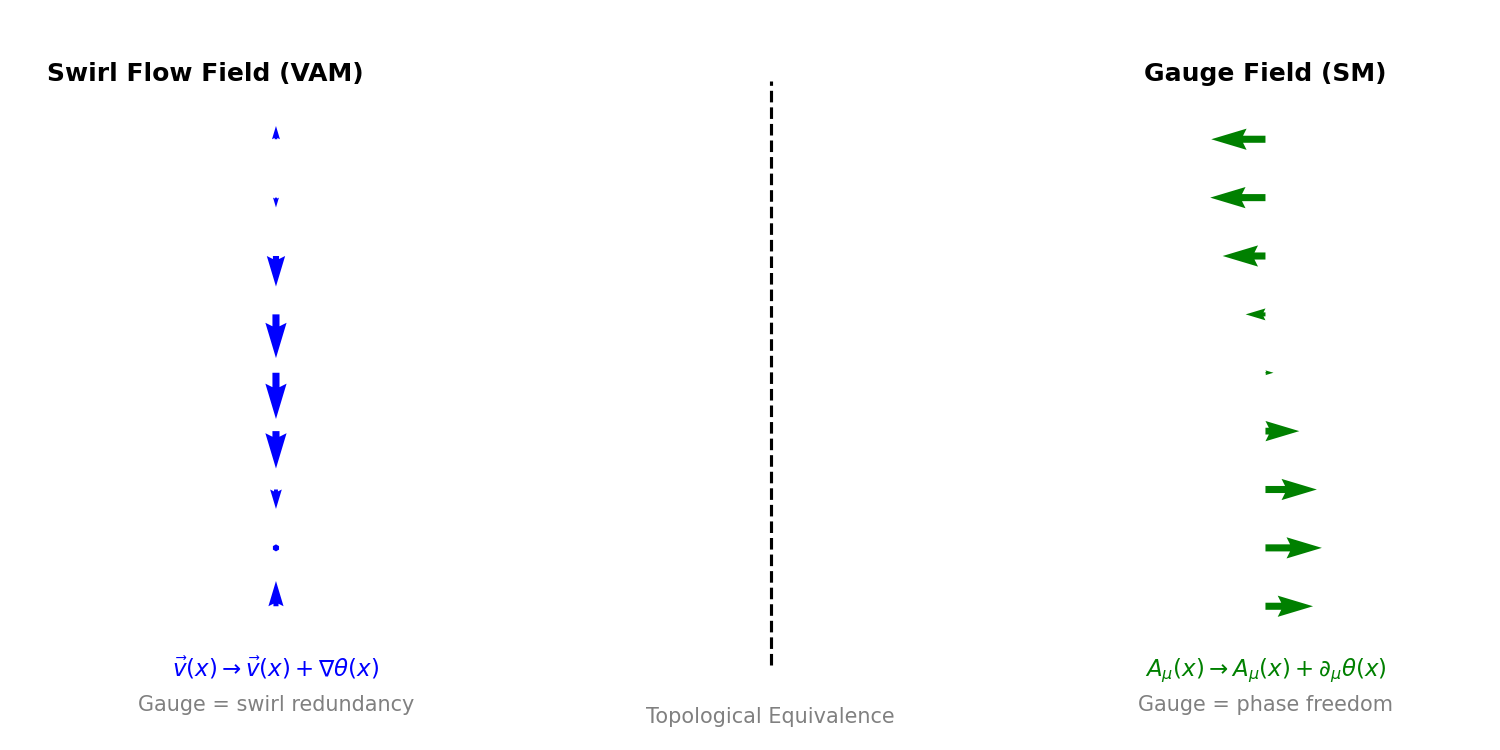
\includegraphics[width=0.95\textwidth]{images/gauge_swirl_equivalence}
    \caption{Analogy between gauge symmetry in the Standard Model and swirl invariance in the Vortex \AE{}ther Model (VAM). Both allow local reparameterizations that leave physical observables unchanged. Gauge symmetry in quantum field theory is structurally equivalent to potential-flow invariance in vortex dynamics.}
    \label{fig:gauge_swirl_equivalence}
\end{figure}

\begin{figure}[H]
    \centering
    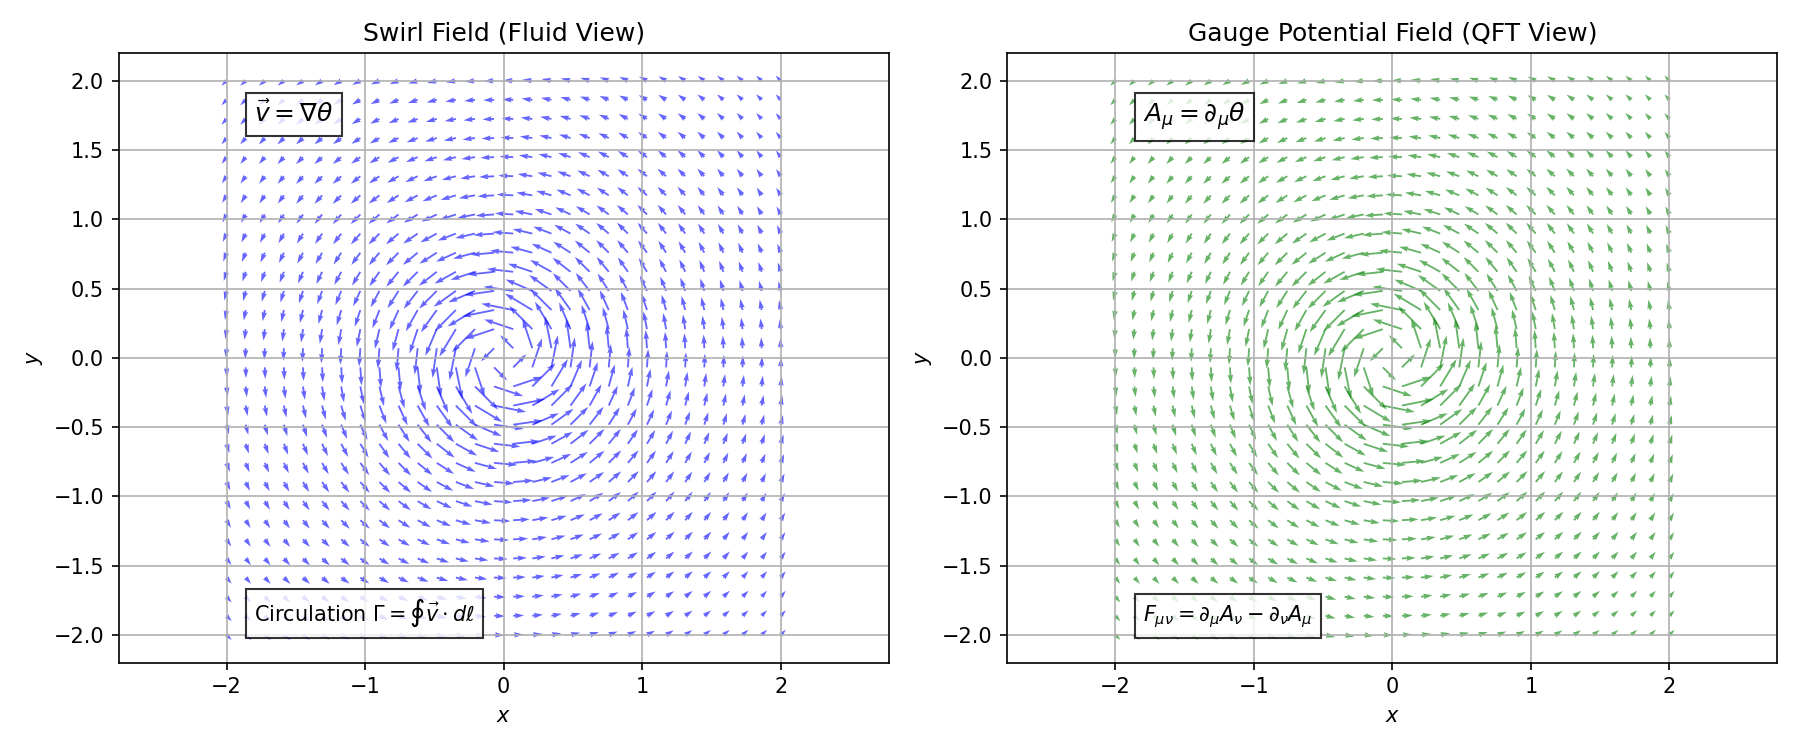
\includegraphics[width=0.9\linewidth]{images/SwirlVSGauge}
    \caption{
        Visual analogy between a fluid swirl field (left) and a gauge potential field in quantum field theory (right).
        Both fields depict circulation around a central core, but the left arises from mechanical vorticity in a compressible \ae{}ther,
        while the right encodes electromagnetic or gauge interaction via abstract potential terms.
        This duality illustrates how local gauge invariance in QFT corresponds to conserved swirl topology in VAM.
    }
    \label{fig:swirl_gauge_analogy}
\end{figure}

\subsection{Fermion Kinetics via Swirl Propagation}
In the hydrodynamic formalism:
\begin{equation}
    \mathcal{L}_{\text{fermion}} = \rho_\text{\ae} C_e \Gamma \left( \psi^* \partial_t \psi - \vec{v} \cdot \nabla \psi \right)
\end{equation}
The convective derivative replaces $D_\mu$, and $\Gamma = 2\pi r_c C_e$ links to the particle's spin-$\tfrac{1}{2}$ topology. Swirl modulates propagation analogous to minimal coupling.

\subsection{Mass from Helicity and Inertia}
The VAM mass term derives from vortex inertia under \ae{}ther drag:
\begin{equation}
    m_f = \frac{\rho_{\ae} \Gamma^2}{3\pi r_c C_e^2} \quad\Rightarrow\quad \mathcal{L}_{\text{mass}} = -m_f \bar{\psi} \psi
\end{equation}
This replaces abstract Yukawa interactions with fluidic resistance to internal swirl flow.

\subsection{Higgs Field as \AE{}ther Compression}
The standard Higgs potential $V(\phi) = -\mu^2|\phi|^2 + \lambda|\phi|^4$ becomes:
\begin{equation}
    V(\rho_\text{\ae}) = \frac{1}{2}K(\rho_\text{\ae} - \rho_0)^2 \quad\text{or}\quad V(\phi) = -\frac{F^{\text{max}}_{\text{\ae}}}{r_c} |\phi|^2 + \lambda |\phi|^4
\end{equation}
$K$ is the \ae{}ther's bulk modulus. The vacuum expectation value corresponds to equilibrium density, leading to spontaneous tension minima that stabilize particle structure.

\subsection{Topological Helicity and Knot Dynamics}
\begin{equation}
    \mathcal{H}_\text{topo} = \int \vec{v} \cdot \vec{\omega} \, dV
\end{equation}
This term tracks conservation of topological linkage and orientation. It becomes significant in processes involving particle transmutation, confinement, or decay.

\subsection{Helicity as a Chern--Simons Analog}
The helicity density term in the Vortex \AE{}ther Model (VAM),
\begin{equation}
\mathcal{L}_{\text{helicity}} = \lambda\, \vec{v} \cdot \vec{\omega},
\end{equation}
serves a central role in encoding the topological complexity of vortex configurations. Here, $\vec{\omega} = \nabla \times \vec{v}$ is the local vorticity field, and $\lambda$ is a coupling constant dependent on the \ae{}ther's inertial density.

However, this term is not merely phenomenological\textemdash it possesses a deep connection with topological field theory, specifically the Chern--Simons action.

In 3D gauge theories, the Abelian Chern--Simons action is given by:
\begin{equation}
S_{\text{CS}} = \int d^3x\, \epsilon^{ijk} A_i \partial_j A_k = \int \vec{A} \cdot (\nabla \times \vec{A})\, d^3x,
\end{equation}
which is formally analogous to the helicity integral in fluid dynamics~\cite{moffatt1969degree,jackiw1990chern}:
\begin{equation}
\mathcal{H} = \int \vec{v} \cdot \vec{\omega}\, d^3x.
\end{equation}

In this analogy, the velocity field $\vec{v}$ plays the role of a gauge potential, and vorticity $\vec{\omega}$ becomes the field strength. This correspondence suggests that helicity is a conserved, quantized topological invariant under the transformation:
\begin{equation}
\theta(\vec{x}) \rightarrow \theta(\vec{x}) + \alpha(\vec{x}) \quad \Rightarrow \quad \vec{v} \rightarrow \vec{v} + \nabla \alpha,
\end{equation}
mirroring a $U(1)$ gauge transformation in QED.

Because the Chern--Simons term is not gauge invariant under large gauge transformations, its quantization ensures that the helicity integral remains invariant up to $2\pi n$ in units of a coupling constant. This provides a natural framework for explaining the quantized linking number $L_k$ of vortex knots in the VAM as a topological charge.

\paragraph{Topological Conservation.}
Because helicity is conserved in ideal fluid flow (barring reconnection events), its inclusion in the Lagrangian provides a natural topological charge for tracking particle identity, decay channels, and symmetry violations. The quantization of $\mathcal{H}_\text{topo} \sim 2\pi L_k$ ensures discrete particle states within continuous field dynamics.

Thus, $\vec{v} \cdot \vec{\omega}$ is not merely a dynamical term, but encodes the fluid analog of a gauge-theoretic topological invariant~\cite{verlinde2021qft}.
